\documentclass{article}
\usepackage{float}
\usepackage[p,osf]{cochineal}
\usepackage[scale=.95,type1]{cabin}
%\usepackage[cochineal,bigdelims,cmintegrals,vvarbb]{newtxmath}
\usepackage{mathpazo}
\usepackage{amsmath}
\usepackage[zerostyle=c,scaled=.94]{newtxtt}
\usepackage{hyperref}
%\usepackage[cal=boondoxo]{mathalfa}
\usepackage{pdflscape}
\usepackage{graphicx}
\usepackage{subcaption}
\usepackage[numbers,sort&compress]{natbib}
\title{Surrogate Model Creation for Constitutive Relations}
\author{Miguel A. Bessa \\ email \href{mailto:M.A.Bessa@tudelft.nl}{M.A.Bessa@tudelft.nl} 
   \and Ozgur Taylan Turan \\ email \href{mailto:O.T.Turan@tudelft.nl}{O.T.Turan@tudelft.nl} }



\begin{document}
\maketitle

Various engineering applications rely on efficient, high performance materials to overcome de-
sign challenges. This high performance can be achieved by engineering micro-heterogenous
materials also known as composites. Since the behavior of composites relies heavily on micro-
scale interactions between different components, modeling macrostructures with fully-represented
microscopic geometry is needed. Thus, the standard finite element modeling approach becomes im-
practical. Computational homogenization, also known as concurrent finite element analysis (FE$^2$),
is a method that is employed to model materials with distinct multi-scaled structure. FE$^2$ employs
the concept of embedding a representative volume element (RVE), at each integration point of the
macro-scale problem and obtaining the macroscopic constitutive behavior through homogenization,
thus bypassing the need to develop a macro-scale constitutive model. Although it succeeds in up-
scaling the microscopic material behavior accurately, this method comes with the major drawback of
being computationally expensive due to its nested structure.

\begin{figure}[!ht]
\begin{subfigure}{.5\textwidth}
  \centering
  % include first image
  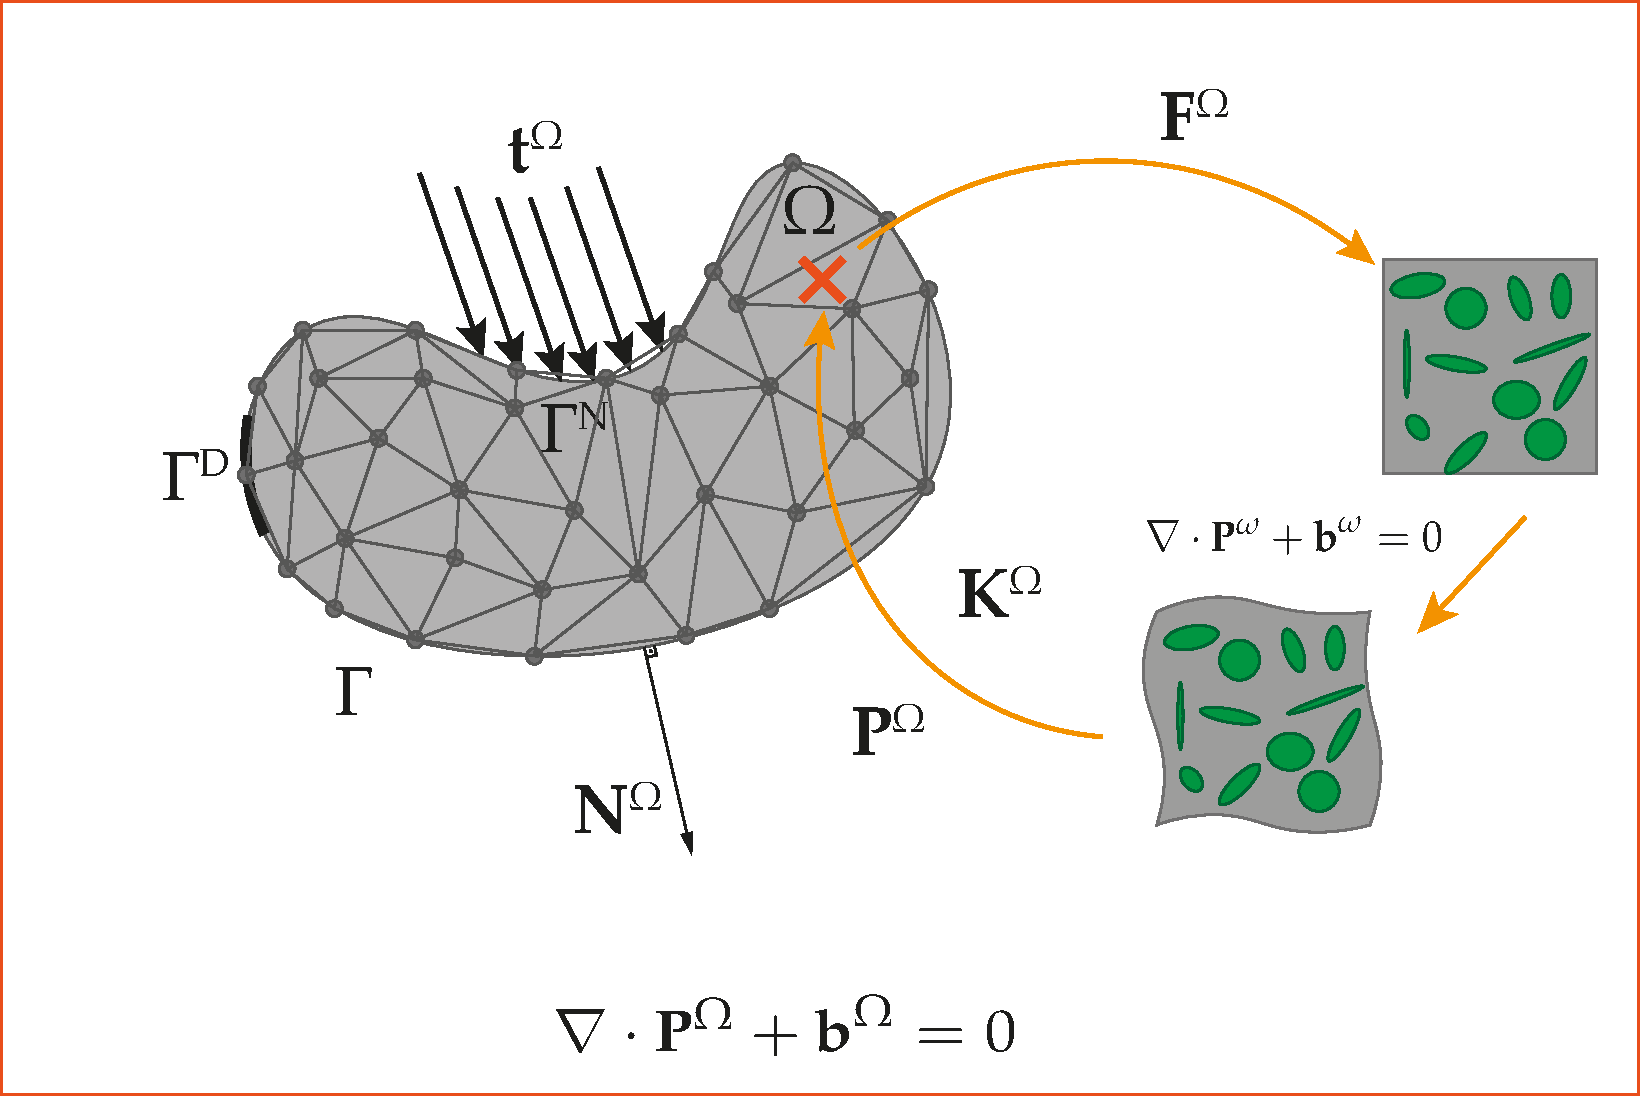
\includegraphics[width=\linewidth]{Figures/FE2}  
  \caption{FE$^2$ Framework}
  \label{fig:fe2}
\end{subfigure}
\begin{subfigure}{.5\textwidth}
  \centering
  % include second image
  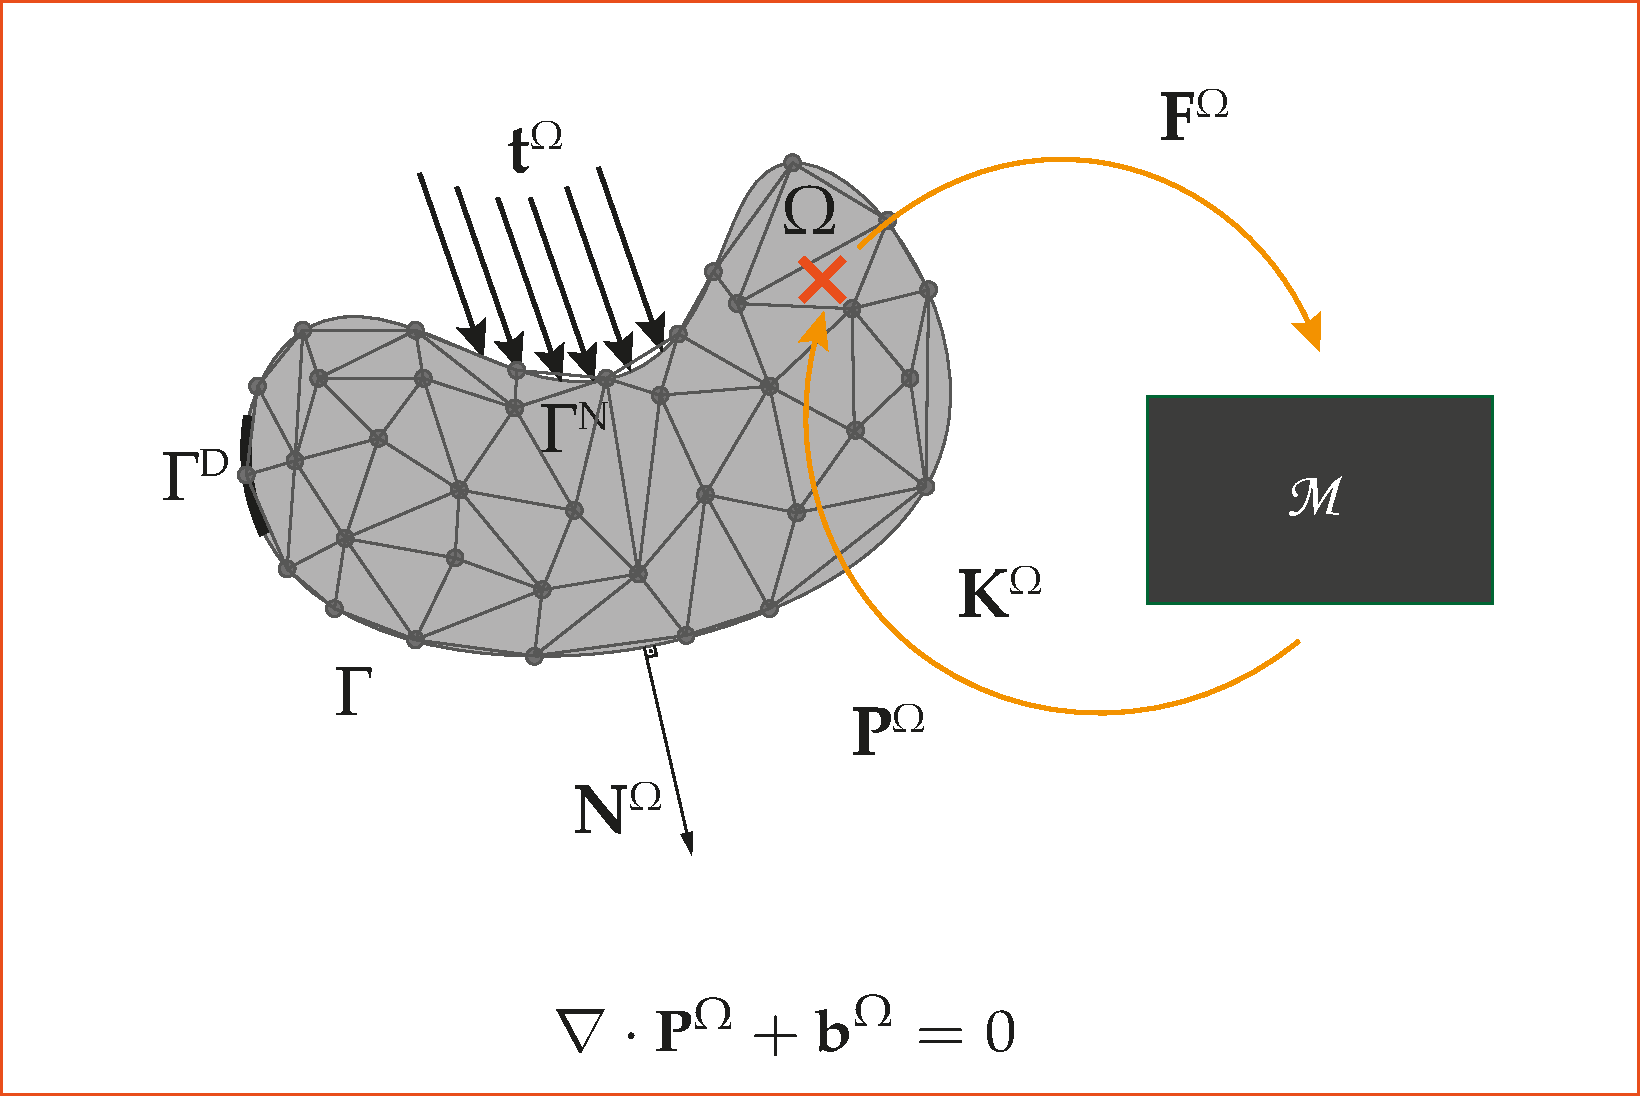
\includegraphics[width=\linewidth]{Figures/FE2-ML}  
  \caption{FE$^2$ with Surrogate ML Model}
  \label{fig:ml}
\end{subfigure}
\caption{Put your caption here}
\label{fig:problem}
\end{figure}

Employing machine learning algorithms to create surrogate constitutive models for microscopic behavior is one possible approach \cite{Bessa2017} to accelerate the multi-scale simulations. This projects aim is to obtain a surrogate constitutive model with a given between macro-scale deformation Gradient Tensor $\mathbf{F}^\Omega$ and the macro-scale second Piola-Kirchhoff Stress Tensor $\mathbf{S}^\Omega$ with additional other geometrical descriptors. In the end, you will be trying to solve a regression problem with $F^\Omega_{11}$, $F^\Omega_{12}$,$F^\Omega_{22}$, $L$, $r$ and $V_f$ as the features and the $S^\Omega_{11}$, $S^\Omega_{12}$, $S^\Omega_{22}$ as the labels. Note that, $L$ is the height of the RVE, $r$ is the radius of the circular inclusions in the RVE and the $V_f$ is the volume fraction which indicates the percentage of the inclusions in the matrix of the composite material. The RVEs under investigation have inclusion modeled by Saint Venant-Kirchhoff Material. All the information related to the dataset generation can be found in the \href{https://colab.research.google.com/drive/10lQ9XWTf4hbG90JCAbc9ZNtRkwQggVYz}{notebook}. Finally you can download the dataset from \href{https://github.com/taylanot/DDSCT/blob/main/examples/dataset.sim}{here}. Note that it is an xarray dataset so you will have to install xarray to your python environment.

\bibliographystyle{unsrtnat}
\bibliography{../../../../../../Dropbox/archive_bib/library.bib}

%Note for Miguel:%
% Hello Miguel, I have prepared this hopefully it will be helpfull. Since I do not know what you expect from students I have not written anything regarding that. My suggestions for their project is as follows:
%-Understand the problem better. (Read your paper!)
%-Read about regression and NNs some of the educated choices you might make!
%Since, I assume they have limited time and compute power, they can fix certain things in the model and try to investigate and report on their findings! My proposal is that, they investigate, 
%-The effect of preprocessing,
%-The effect of activation function,
%-The effect of optimization algorithm,
%-The effect of batch size, and
%-The effect of Architecture selection.
%After they are done with small investigation of these they can try to find a good model for the problem that they have!
%-As a bonus, other models and the effect of regularization $L_2$ and $L_1$ can be added!
%-Please let me know in-advance what you would like me to do explicitly other wise I get quite stressed out. Thank you!


\end{document}
